\documentclass[11pt]{article}
\linespread{1.15}

%%%%%%%%%%%%%%Include Packages%%%%%%%%%%%%%%%%%%%%%%%%%%
\usepackage{xcolor}
\usepackage{mathtools}
\usepackage[a4paper, total={6in, 8in}, margin=1.25in]{geometry}
\usepackage{amsmath}
\usepackage{amssymb}
\usepackage{paralist}
\usepackage{rsfso}
\usepackage{amsthm}
\usepackage{wasysym}
\usepackage[inline]{enumitem}   
\usepackage{hyperref}
\usepackage{tocloft}
\usepackage{wrapfig}
\usepackage{titlesec}
\usepackage{colortbl}
\usepackage{stackengine} 
%%%%%%%%%%%%%%%%%%%%%%%%%%%%%%%%%%%%%%%%%%%%%%%%%%%%%%%%


%%%%%%%%%%%%%%%Chapter Setting%%%%%%%%%%%%%%%%%%%%%%%%%%
\definecolor{gray75}{gray}{0.75}
\newcommand{\hsp}{\hspace{20pt}}
\titleformat{\chapter}[hang]{\Huge\bfseries}{\thechapter\hsp\textcolor{gray75}{$\mid$}\hsp}{0pt}{\Huge\bfseries}
%%%%%%%%%%%%%%%%%%%%%%%%%%%%%%%%%%%%%%%%%%%%%%%%%%%%%%%%

%%%%%%%%%%%%%%%%%Theorem environments%%%%%%%%%%%%%%%%%%%
\newtheoremstyle{break}
  {\topsep}{\topsep}%
  {\itshape}{}%
  {\bfseries}{}%
  {\newline}{}%
\theoremstyle{break}
\theoremstyle{break}
\newtheorem{axiom}{Axiom}
\newtheorem{thm}{Theorem}[section]
\renewcommand{\thethm}{\arabic{section}.\arabic{thm}}
\newtheorem{lem}{Lemma}[thm]
\newtheorem{cor}{Corollary}[thm]
\newtheorem{defn}{Definition}[thm]
\newenvironment{indEnv}[1][Proof]
  {\proof[#1]\leftskip=1cm\rightskip=1cm}
  {\endproof}
%%%%%%%%%%%%%%%%%%%%%%%%%%%%%%%%%%%%%%%%%%%%%%%%%%%%%%


%%%%%%%%%%%%%%%%%%%%%%%Integral%%%%%%%%%%%%%%%%%%%%%%%
\def\upint{\mathchoice%
    {\mkern13mu\overline{\vphantom{\intop}\mkern7mu}\mkern-20mu}%
    {\mkern7mu\overline{\vphantom{\intop}\mkern7mu}\mkern-14mu}%
    {\mkern7mu\overline{\vphantom{\intop}\mkern7mu}\mkern-14mu}%
    {\mkern7mu\overline{\vphantom{\intop}\mkern7mu}\mkern-14mu}%
  \int}
\def\lowint{\mkern3mu\underline{\vphantom{\intop}\mkern7mu}\mkern-10mu\int}
%%%%%%%%%%%%%%%%%%%%%%%%%%%%%%%%%%%%%%%%%%%%%%%%%%%%%%



\newcommand{\R}{\mathbb{R}}
\newcommand{\N}{\mathbb{N}}
\newcommand{\Z}{\mathbb{Z}}
\newcommand{\Q}{\mathbb{Q}}
\newcommand{\C}{\mathbb{C}}
\newcommand{\T}{\mathcal{T}}
\newcommand{\M}{\mathcal{M}}
\newcommand{\Symm}{\text{Symm}}
\newcommand{\Alt}{\text{Alt}}
\newcommand{\Int}{\text{Int}}
\newcommand{\Bd}{\text{Bd}}
\newcommand{\Power}{\mathcal{P}}
\newcommand{\ee}[1]{\cdot 10^{#1}}
\newcommand{\spa}{\text{span}}
\newcommand{\sgn}{\text{sgn}}
\newcommand{\degr}{\text{deg}}
\newcommand{\pd}{\partial}
\newcommand{\that}[1]{\widetilde{#1}}
\newcommand{\lr}[1]{\left(#1\right)}
\newcommand{\vmat}[1]{\begin{vmatrix} #1 \end{vmatrix}}
\newcommand{\bmat}[1]{\begin{bmatrix} #1 \end{bmatrix}}
\newcommand{\pmat}[1]{\begin{pmatrix} #1 \end{pmatrix}}
\newcommand{\rref}{\xrightarrow{\text{row\ reduce}}}
\newcommand{\txtarrow}[1]{\xrightarrow{\text{#1}}}
\newcommand\oast{\stackMath\mathbin{\stackinset{c}{0ex}{c}{0ex}{\ast}{\Circle}}}
\newcommand{\txt}{G. Grimmett and D. Stirzaker's \textit{Probability and Random Processes}}

\newcommand{\note}{\color{red}Note: \color{black}}
\newcommand{\remark}{\color{blue}Remark: \color{black}}
\newcommand{\example}{\color{green}Example: \color{black}}
\newcommand{\exercise}{\color{green}Exercise: \color{black}}

%%%%%%%%%%%%%%%%%%%%%%Roman Number%%%%%%%%%%%%%%%%%%%%%%%
\makeatletter
\newcommand*{\rom}[1]{\expandafter\@slowromancap\romannumeral #1@}
\makeatother
%%%%%%%%%%%%%%%%%%%%%%%%%%%%%%%%%%%%%%%%%%%%%%%%%%%%%%%%%

%%%%%%%%%%%%%table of contents%%%%%%%%%%%%%%%%%%%%%%%%%%%%
%\setlength{\cftchapindent}{0em}
%\cftsetindents{section}{2em}{3em}
%
%\renewcommand\cfttoctitlefont{\hfill\huge\bfseries}
%\renewcommand\cftaftertoctitle{\hfill\mbox{}}
%
%\setcounter{tocdepth}{2}
%%%%%%%%%%%%%%%%%%%%%%%%%%%%%%%%%%%%%%%%%%%%%%%%%%%%%%%%%%


%%%%%%%%%%%%%%%%%%%%%Footnotes%%%%%%%%%%%%%%%%%%%%%%%%%%%
\newcommand\blfootnote[1]{%
  \begingroup
  \renewcommand\thefootnote{}\footnote{#1}%
  \addtocounter{footnote}{-1}%
  \endgroup
}
%%%%%%%%%%%%%%%%%%%%%%%%%%%%%%%%%%%%%%%%%%%%%%%%%%%%%%%%%

%%%%%%%%%%%%%%%%%%%%%Section%%%%%%%%%%%%%%%%%%%%%%%%%%%%%
\makeatletter
\def\@seccntformat#1{%
  \expandafter\ifx\csname c@#1\endcsname\c@section\else
  \csname the#1\endcsname\quad
  \fi}
\makeatother
%%%%%%%%%%%%%%%%%%%%%%%%%%%%%%%%%%%%%%%%%%%%%%%%%%%%%%%%%

%%%%%%%%%%%%%%%%%%%%%%%%%%%%%%%%%%%Enumerate%%%%%%%%%%%%%%
\makeatletter
% This command ignores the optional argument 
% for itemize and enumerate lists
\newcommand{\inlineitem}[1][]{%
\ifnum\enit@type=\tw@
    {\descriptionlabel{#1}}
  \hspace{\labelsep}%
\else
  \ifnum\enit@type=\z@
       \refstepcounter{\@listctr}\fi
    \quad\@itemlabel\hspace{\labelsep}%
\fi}
\makeatother
\parindent=0pt
%%%%%%%%%%%%%%%%%%%%%%%%%%%%%%%%%%%%%%%%%%%%%%%%%%%%%%%%%%



\begin{document}

	\begin{titlepage}
		\begin{center}
			\vspace*{0.5cm}
			\LARGE \color{black}
				\textbf{The Markov Chain Monte Carlo Method \\and its Application in Astrophysics}\\
			\vspace{1.5cm}			
			\Large \color{gray}
			Final Project for Math 525 - Probability Theory\\
			Professor Dan Burns
			\color{black}
			\vspace{3cm}			
			
			\vspace{6cm}
			\LARGE
			    \textbf{Jinyan Miao and Chi Han} \\
			    \vspace{0.5cm}
				\LARGE Fall 2023\\
			\vspace{1cm}

		\vspace*{\fill}
		\end{center}			
	\end{titlepage}


\newpage
\tableofcontents
\hfill\break
\noindent\rule{8cm}{1pt}
\section{Introduction}
{}\qquad In the field of astrophysics, one key research interest lies in using experimental data to constrain cosmological parameters in the Lambda Cold Dark Matter ($\Lambda$CDM) model, a mathematical model of the Big Bang theory. This involves computing the likelihood of the observed data given the model with various sets of cosmological parameters.\\


{}\qquad First we consider a simple problem: Given the occurrence of some data, we are interested in calculating the conditional probability in a given multidimensional probability space. This is now always feasible due to the computation cost of mapping out a potentially huge parameter space. For instance, if we have $10$ cosmological parameters, each viewed as discrete random variables and each takes $50$ different values, then we first need to perform $20^{50} \sim 10^{65}$ calculations to obtain the joint distribution. If each calculation further involves performing integration to evaluate, say, the luminosity distance in the model, the computation cost of mapping out the parameter space is significant, and it increases rapidly as one increases the number of cosmological parameters considered. Thus we seek methods to simplify our calculations and analysis. The Markov Chain Monte Carlo (MCMC) method is utilized to generate samples from the posterior distribution of interest, facilitating the evaluation of quantities such as expectation, median, and variance of the distribution. The MCMC method turns out to be particularly beneficial in expediting the analysis of cosmological parameters.\\

{}\qquad In this text, we will start by giving theoretical construction of the MCMC method and algorithms of constructing the Markov chains, then we will apply it to constrain the cosmological parameters $\Omega_m$, $\Omega_{\Lambda}$, and $w$ in their joint probability space using the observed data on the apparent brightness versus redshift of a uniform set of Type Ia Supernovae \cite{U21}, and reproduce the results in the publications \cite{U21} and \cite{U2}.


\section{Markov Chain Monte Carlo}
\subsection{Motivation}
{}\qquad Given an observed evidence $X$, for $\theta$ in the parameter space $\Omega$, one is interested in calculating the posterior distribution
\begin{align}
p(\theta | X) = \frac{p(X|\theta) \, p(\theta)}{p(X)}\,.
\end{align}
Here $p(X|\theta)$ is the likelihood, which can usually be calculated using some model. We call $p(\theta)$ the prior, and the normalization constant $p(X)$ the marginal likelihood. As mentioned in the Introduction section, the computation cost of the normalization constant $p(X)$, even in the case of $X$ is finite,
\begin{align*}
p(X) = \sum_{\psi \in \Omega} p(X|\psi) \, p(\psi)\,,
\end{align*}
can be significant. In the case where $X$ is continuous, 
\begin{align}
p(X) = \int_{\psi \in \Omega} p(X|\psi)\, p(\psi)
\end{align}
is much more difficult to evaluate as the space $\Omega$ can be potentially huge. To estimate the posterior $p(\theta|X)$, the Markov Chain Monte Carlo methods (MCMC) resolve the issue of computation cost by avoiding calculating the normalization constant $p(X)$.\\

${}$\qquad We will construct a Markov chain having the properties that (a) the chain has a unique stationary distribution as the posterior distribution, and (b) the transition probabilities of the chain have a simple form. Here (b) ensures the simulation easiness of the chain \cite{txt}. To construct the Markov chain, given an initial step, the next step is drawn from a proposed distribution. The draw of the next step will depend only on the state of the current step, hence the chain is Markov. We apply further conditions such that the chain will have a unique stationary distribution. In particular, not all draws are used, we will set up the acceptance criteria for each draw based on comparing the successive states with respect to a target distribution to ensure that the stationary distribution is the posterior distribution of interest \cite{Duke}. With this procedure, the target distribution only needs to be proportional to the posterior distribution, such that the evaluation of Eq.\ (2) is avoided.
 

\subsection{The Metropolis-Hastings Algorithm}
${}$\qquad There are many different ways to construct MCMC, we start with the simple one, the Metropolis-Hastings random walk algorithm.\\

${}$\qquad Here we will denote the proposal distribution as $q(\theta | \theta')$. The target distribution, which is only required to be proportional to the posterior distribution, can be chosen easily, for instance,
\begin{align*}
g(x) = p(X|x) \, p(x)
\end{align*}
would satisfy the requirement according to Eq.\ (1). Note that even though $g(x)$ is called a distribution, it needs not to be normalized. Consider we are given the probability space $\Omega$, and an initial state $\theta_0 \in \Omega$. The Metropolis-Hastings algorithm proceeds as follows:
\begin{enumerate}[topsep=3pt,itemsep=-1ex,partopsep=1ex,parsep=1ex]
\item We propose a new state $\theta_p = \theta_0 + \Delta \theta$, where $\Delta \theta$ is sampled from the proposal distribution $q(\theta_p|\theta_0)$.
\item Then we calculate the ratio according to the posterior distribution $p(\theta|X)$,
\begin{align}
\rho = \frac{p(\theta_p|X)}{p(\theta_0|X)} \frac{q(\theta_0|\theta_p)}{q(\theta_p|\theta_0)}= \frac{g(\theta_p)}{g(\theta_0)}\frac{q(\theta_0|\theta_p)}{q(\theta_p|\theta_0)}    =
\frac{p(X|\theta_p)\, p(\theta_p)}{p(X|\theta_0)\, p(\theta_0)}
\frac{q(\theta_0|\theta_p)}{q(\theta_p|\theta_0)}  \,,
\end{align}
where the factor $q(\theta_0|\theta_p )/q(\theta_p|\theta_0)$, calculated from the proposal distribution, is appended to ensure stationary distribution as we shall discuss next. In the case where the proposal distribution is symmetric, such as using the normal distribution as proposal distribution, this factor is simply one. 
\item Next we define the first step $\theta_1$. If $\rho \geq 1$, then $\theta_1 = \theta_p$. If $\rho < 1$, then we define $\theta_1 = \theta_p$ with probability $\rho$, and $\theta_1 = \theta_0$ with probability $1-\rho$.
\item We repeat (1.) through (3.) to define the steps $\theta_2, \theta_3,\cdots$ in the chain. 
\end{enumerate}

${}$\qquad Here we will develop some intuition about the procedure. In the case of having symmetric proposal distribution, according to Eq.\ (3), $\rho > 1$ whenever $p(\theta_p|X) > p(\theta_0|X)$. That is, we move to $\theta_1 = \theta_p$ from $\theta_0$ with probability $1$ when $\theta_p$ is \textit{preferred} by the observed evidence $X$. On the other hand, if we set $\theta_1 = \theta_0$ whenever $\rho = 0$, it is possible that we will get stuck at a local mode of the target distribution $g(x)$, so we occasionally accept moves to states $\theta_p$ in the region with lower probability density. The key observation here is that, after some burn-in initial steps, the chain $\theta_i$ is expected to spend its time walking in places proportional to the density of the posterior distribution, and we have avoided the computation cost of computing Eq.\,(2). \\

${}$\qquad 
Note further that we have imposed the detailed balance criterion when constructing the chain. To see this, the detailed balance criterion states that the probability of being in state $\theta$ and moving to state $\theta'$ must be the same as the probability of being in state $\theta'$ moving to state $\theta$. In other words, we require
\begin{align*}
{p(\theta|X)\, f(\theta\to\theta')}={p(\theta'|X)\, f(\theta'\to\theta)}\,,
\end{align*}
where $p(\theta|X)$ is the posterior distribution and $f(\theta\to\theta')$ is the probability of going from state $\theta$ to $\theta'$. Rearranging we obtain
\begin{align}
\frac{p(\theta|X)}{p(\theta'|X)} = \frac{f(\theta'\to\theta)}{f(\theta\to\theta')}\,.
\end{align}
In step (3.) in the algorithm we have criteria for accepting the proposed movement, we denote the probability of the proposed movement being accepted as $a(\theta_0\to \theta_p)$, then combine with Eq.\ (4) we obtain
\begin{align*}
\frac{p(\theta_p|X)}{p(\theta_0|X)} = \frac{a(\theta_0\to\theta_p)\, q(\theta_p| \theta_0)}{a(\theta_p\to\theta_0)\, q(\theta_0|\theta_p)}\,.
\end{align*}
Rearranging we obtain
\begin{align*}
\frac{a(\theta_0\to\theta_p)}{a(\theta_p\to\theta_0)}
= \frac{p(\theta_p|X)}{p(\theta_0|X)} \frac{q(\theta_0|\theta_p)}{q(\theta_p|\theta_0)}\,,
\end{align*}
which gives rise to the factor $q(\theta_0|\theta_p)/q(\theta_p|\theta_0)$ we appended in step (2.) of the algorithm, and thus the acceptance probability that meets such a condition is
\begin{align}
a(\theta_0 \to \theta_p) = \min\left(1, \,  \frac{p(\theta_p|X)}{p(\theta_0|X)} \frac{q(\theta_0|\theta_p)}{q(\theta_p|\theta_0)}\right) = \min\left( 1 , \rho\right)\,.
\end{align}

${}$\qquad Here we also give a brief justification for the convergence of the chain that we construct. First notice that the chain is Markov as the transition criterion to the next step only depends on the property of the current step according to Eq.\ (5). For finite state space $\Omega$, irreducibility and aperiodicity of the chain guarantee its convergence to a stationary distribution by Theorems in \txt\ \cite{txt}. For infinite state space, a condition of positive recurrence shall be added. It is not hard to observe from the design of the algorithm that all those requirements are met, and thus our Markov chain converges to a stationary distribution $\pi$. While in order to ensure $\pi$ is $p(\theta|X)$, one can show that a sufficient but not necessary condition to have $\pi = p(\theta|X)$ is the detailed balance criterion that we have just discussed \cite{ML}.\\

${}$\qquad Lastly, we notice that the step size generated by the proposal distribution is too small, the random walk might stuck at a local mode of the posterior distribution. If the step size is too large, there is great inefficiency due to a high rejection rate \cite{ML}. As illustrated in the following figures, proposal distribution is the normal distribution with standard deviation $\sigma^*$.

\begin{center}
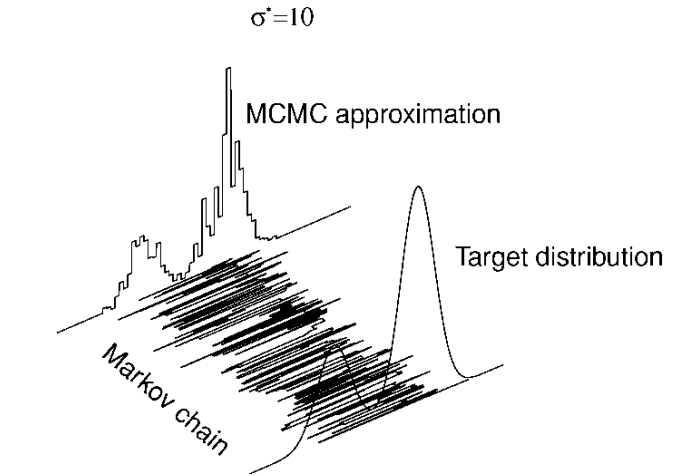
\includegraphics[scale=0.55]{MCMC}\\

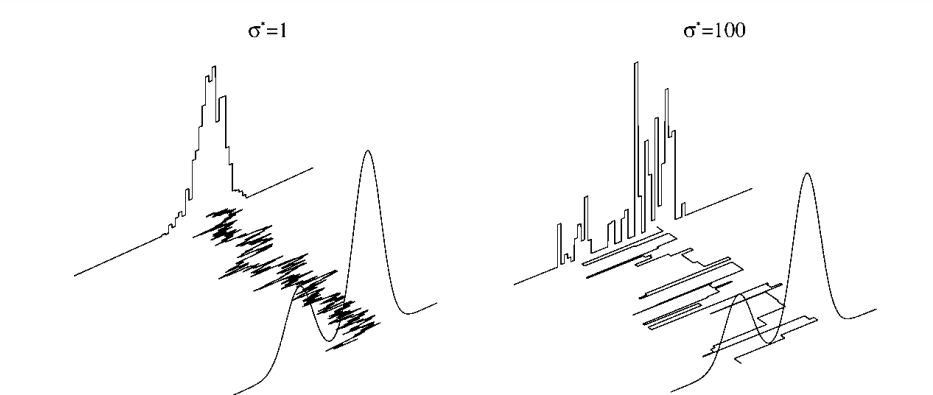
\includegraphics[scale=0.68]{MCMC-sample}\\

Figure 1. Approximations obtained using the Metropolis-Hastings algorithm with three normal proposal distributions of different variances \cite{ML}.\\
\end{center}


\subsection{Other MCMC Algorithms}
${}$\qquad Other than the Metropolis-Hastings algorithm, many more algorithms can be used to generate a Markov chain, such as the Gibbs sampling and the slice sampling. Here we will give a brief introduction to these two processes.\\

${}$\qquad The Gibbs sampling deals with a vector of parameters, that is $\vec{\theta} = (\theta_1,\theta_2,\cdots, \theta_k)$. Suppose again we want to estimate the posterior distribution $p(\theta|X)$, and assume that all of the following conditional distributions are well defined up to a normalization constant:
\begin{align*}
p(\theta_1 | \theta_2,\theta_3,\cdots,\theta_k,X) \,,\quad
p(\theta_2 | \theta_1,\theta_3,\cdots,\theta_k,X) \,,\quad
\cdots\,,\quad
p(\theta_k | \theta_1,\theta_2,\cdots,\theta_{k-1},X)\,.
\end{align*}
Then, given an initial step $\vec{\theta}^0 = (\theta_1^0,\theta_2^0,\cdots, \theta_k^0)$ of the chain, with the proposed step denoted as $\vec{\theta}^1=(\theta_1^1,\theta_2^1,\cdots, \theta_k^1)$, the component $\theta_i^1$ is sampled from the distribution
\begin{align*}
p(\theta_i^1 |\theta_1^1, \theta_2^1, \cdots, \theta_{i-1}^1, \theta_{i+1}^0, \theta_{i+2}^0,\cdots \theta_k^0, X)\,. 
\end{align*}
The proposed step has an acceptance probability being $1$, that is $\vec{\theta}^1$ is exactly the next step. Steps $\vec{\theta}^2, \vec{\theta}^3, \cdots$ are sampled similarly. We see from here that the Gibbs sampling can be viewed as a Metroplish-Hasting algorithm with a special proposal distribution and with the acceptance probability of the proposed movement being $1$. Gibbs sampling is believed to be very efficient in terms of programming when dealing with vector parameter $\vec{\theta}$, as it does not involve any tuning process \cite{Duke}.\\

${}$\qquad The slice sampling is a little more complicated. Suppose one wants to sample from the posterior distribution $f(\theta) = p(\theta|X)$. In the simplest form of slice sampling, one samples uniformly under the curve $f(\theta)$ with acceptance probability $1$. That is, given an initial step $\theta_0$ that satisfies $f(\theta_0) > 0$, we define steps in the chain utilizing the following procedure:
\begin{enumerate}[topsep=3pt,itemsep=-1ex,partopsep=1ex,parsep=1ex]
\item We sample a value $\phi_0$ uniformly between $0$ and $f(\theta_0)$, 
\item then we draw a horizontal line under the curve of $f$ at vertical position $\phi_0$.
\item From the line segment(s) obtained in step (2.), we sample a value of $\theta_1$ uniformly. 
\item Repeat from step (1.) to obtain steps $\theta_2$, $\theta_3$, $\cdots$.  
\end{enumerate}
Again, this algorithm can be used to sample from the area under any reasonable curve, regardless of its normalization. Compared to the Metropolis-Hastings algorithm, which is sensitive to step size, the slice sampling automatically adjusts the step size to match the local shape of the density function.

\section{Application of MCMC in Astrophysics}
\subsection{The $\Lambda$CDM Model}
${}$\qquad Our universe can be characterized by the Robertson-Walker metric
\begin{align}
-c^2\, d\tau^2 = -c^2 \,dt^2 + a(t)^2\, d\Sigma^2\,,
\end{align}
where $\tau$ is the proper time, $c$ is the speed of light, $t$ is the coordinate time, $\Sigma$ ranges over a 3-dimensional space of uniform curvature, and $a(t)$ is known as the scale factor of the universe. Here $a(t)$ can be used to describe the expansion of the universe. One quantity that the cosmological community is interested in is the time-dependent Hubble parameter $H(t)$, defined as
\begin{align*}
H(t) \coloneqq \frac{\dot{a}}{a} = \frac{da}{dt}\, \frac{1}{a}\,.
\end{align*}
Note that $a$ is in fact defined relative to the present time, so $a_0 = a(t_0) = 1$, where the subscript $0$ denotes the present-day values. The scale factor $a$ is also related to the observed redshift $z$ of light emitted at time $t_{\text{em}}$ by $a(t_{\text{em}}) = (1+z)^{-1}$. Using the Friedmann equation, one finds that we have
\begin{align*}
H(a) &= H_0\sqrt{\Omega_m a^{-3} + \Omega_r a^{-4} + \Omega_k a^{-2} + \Omega_\Lambda a^{-3(1+w)}}\,,\\
H(z) &= H_0\sqrt{\Omega_m (1+z)^{3} + \Omega_r (1+z)^{4} + \Omega_k (1+z)^{2} + \Omega_\Lambda (1+z)^{3(1+w)}}\,, \tag{7}
\end{align*}
\setcounter{equation}{7}

where $w$ is the equation of state parameter of dark energy. The various 
$\Omega$ parameters add up to $1$ by construction. Measuring the basic values of the cosmological parameters $\Omega_M, \, H_0,\, w$ has always been an important goal for the astrophysics community, and there have been numerous studies on it since the measurement of the Hubble constant in 1929. The general definition of the luminosity distance for a flat universe is given by
\begin{align}
d_L= \frac{c(1+z)}{H_0}\int_0^z \frac{dz'}{H(z')}\,.
\end{align}
Lastly, we define the distance modulus,
\begin{align}
m(d_L) = 5\, \log_{10}\left(\frac{d_L}{10\, [\text{pc}]}\right)\,.
\end{align}
${}$\qquad Luminosity distance is useful in measuring the cosmological parameters. In the experiment, we use the standard candles Type Ia supernova to obtain data on distance modulus. By constructing a model of posterior distribution $p(\theta|X)$, with $\theta$ being the cosmological parameters and $X$ being the experimentally observed distance modulus, we are able to constrain the cosmological parameters that the distance modulus is dependent on via Eq.\ (7), (8) and (9).

\subsection{Analysis on Union 2.1 Supernovae Data}
${}$\qquad In this section, we will constrain cosmological parameters $\Omega_M, w, H_0$ using data of a set of Type Ia Supernovae, which are distant explosions of stars that are nearly standard candles – events with nearly uniform intrinsic luminosity \cite{U21}. Cosmologists use them to measure distance as a function of redshift, thereby constraining cosmological parameters.\\

${}$\qquad We are using the Union 2.1 data \cite{U21}, which contains the data of 580 supernovae (SN) data. The data contains columns of SN names, redshift, distance modulus, and distance modulus error. First we define the likelihood $\mathcal{L}$,
\begin{align}
\mathcal{L} \propto \exp\left( -\chi^2/2\right)\,,
\end{align}
where $\chi^2$ is the normalized square distance between the SN data and the model, 
\begin{align*}
\chi^2 = \sum_{i=1}^{N_{\text{SN}}} \left( \frac{m_i - \hat{m}(z_i,\vec{p})}{\sigma_i} \right)^2\,.
\end{align*}
Here $N_{\text{SN}}=580$ is the number of SN data points, $m_i$ is the distance modulus in the data, $\hat{m}(z_i,\vec{p})$ is the distance modulus predicted by the model with redshift $z_i$ and cosmological parameters $\vec{p} = (\Omega_M, w, H_0)$ via Eq.\ (7), (8), and (9), and $\sigma_i$ is the error of the distance modulus in the data. \\

${}$\qquad Now we rewrite Eq.\ (1) in the following way,
\begin{align}
p(\vec{p}\,|X) \propto \mathcal{L}(\vec{p})\cdot p(\vec{p})\,,
\end{align}
where $X$ denotes the observed data. We have omitted all proportional factors as we are not interested in those factors and computing them involves mapping out the huge parameter space $\{\Omega_m\} \times \{w\} \times \{H_0\}$. For instance, here we are considering the free cosmological parameters $\Omega_m,w, H_0$. If for each of them we consider $100$ different values, then a total of $100^3 \sim 10^{6}$ integrals in Eq.\ (8) need to be computed. This number will increase significantly if we further let $\Omega_r, \Omega_k, \Omega_\Lambda$ be free variables. Since the proportional constant does not affect the sample result in the MCMC method as we have discussed in the previous sections, we simply drop those proportional constants. Furthermore, the prior distribution $p(\vec{p})$ in Eq.\ (11) is not normalized, as the normalization only gives a proportional constant that can be dropped. With some realistic consideration of the range of the parameters, $p(\vec{p})$ takes the following form:
\begin{align*}
p(\vec{p}) = \begin{cases}
1 & \Omega_m\in (0,1), \ H_0\in (50,100),\ w\in (-1.6, 0) \\
0 & \text{otherwise}
\end{cases}\ .
\end{align*}

${}$\qquad Now we proceed with the standard procedure in the MCMC methods to sample the posterior, or equivalently, according to Eq.\ (11), sample the likelihood within the parameter space of interest. Our algorithm for constructing the Markov chain proceeds as follows:
\begin{enumerate}
\item Select a starting point $\vec{p} = (\Omega_m, w, H_0)$ for the chain.
\item Let the normal distribution be the proposal distribution. That is, we draw a sample $|\delta \vec{p}| \in \mathcal{N}(0,\sigma)$ with $\sigma$ being chosen carefully.
\item We define the acceptance criteria. If $\mathcal{L}(\vec{p}+\delta \vec{p}) \geq \mathcal{L}(\vec{p})$, we accept the proposed movement, so $\vec{p} \to \vec{p} + \delta \vec{p}$ with probability $1$. If $\mathcal{L}(\vec{p} + \delta \vec{p}) < \mathcal{L}(\vec{p})$, we accept the proposed movement with probability $\mathcal{L}(\vec{p}+\delta\vec{p})/\mathcal{L}(\vec{p})$, and otherwise reject the proposed movement and stay at the point $\vec{p}$.
\end{enumerate} 
This procedure is in fact the Metropolis-Hasting algorithm discussed in the previous section. The $\sigma$ in the proposal distribution is chosen based on analysis in {Ref.\ \cite{U21}}. \\

${}$\qquad In our analysis, we used 20 walkers with randomly selected starting points in the parameter space of interest, and a burn-in step of $40$. The walkers moved $2000$ steps after removing the burn-ins. Figure 2 shown in the following serves as a visualization of the position of the walkers in the 2000 steps, with the $40$ burn-in steps being omitted. We see that the walkers spend their time bouncing around the medium after the burn-ins, as expected from the theory of the Metropolis-Hastings algorithm.


\begin{center}
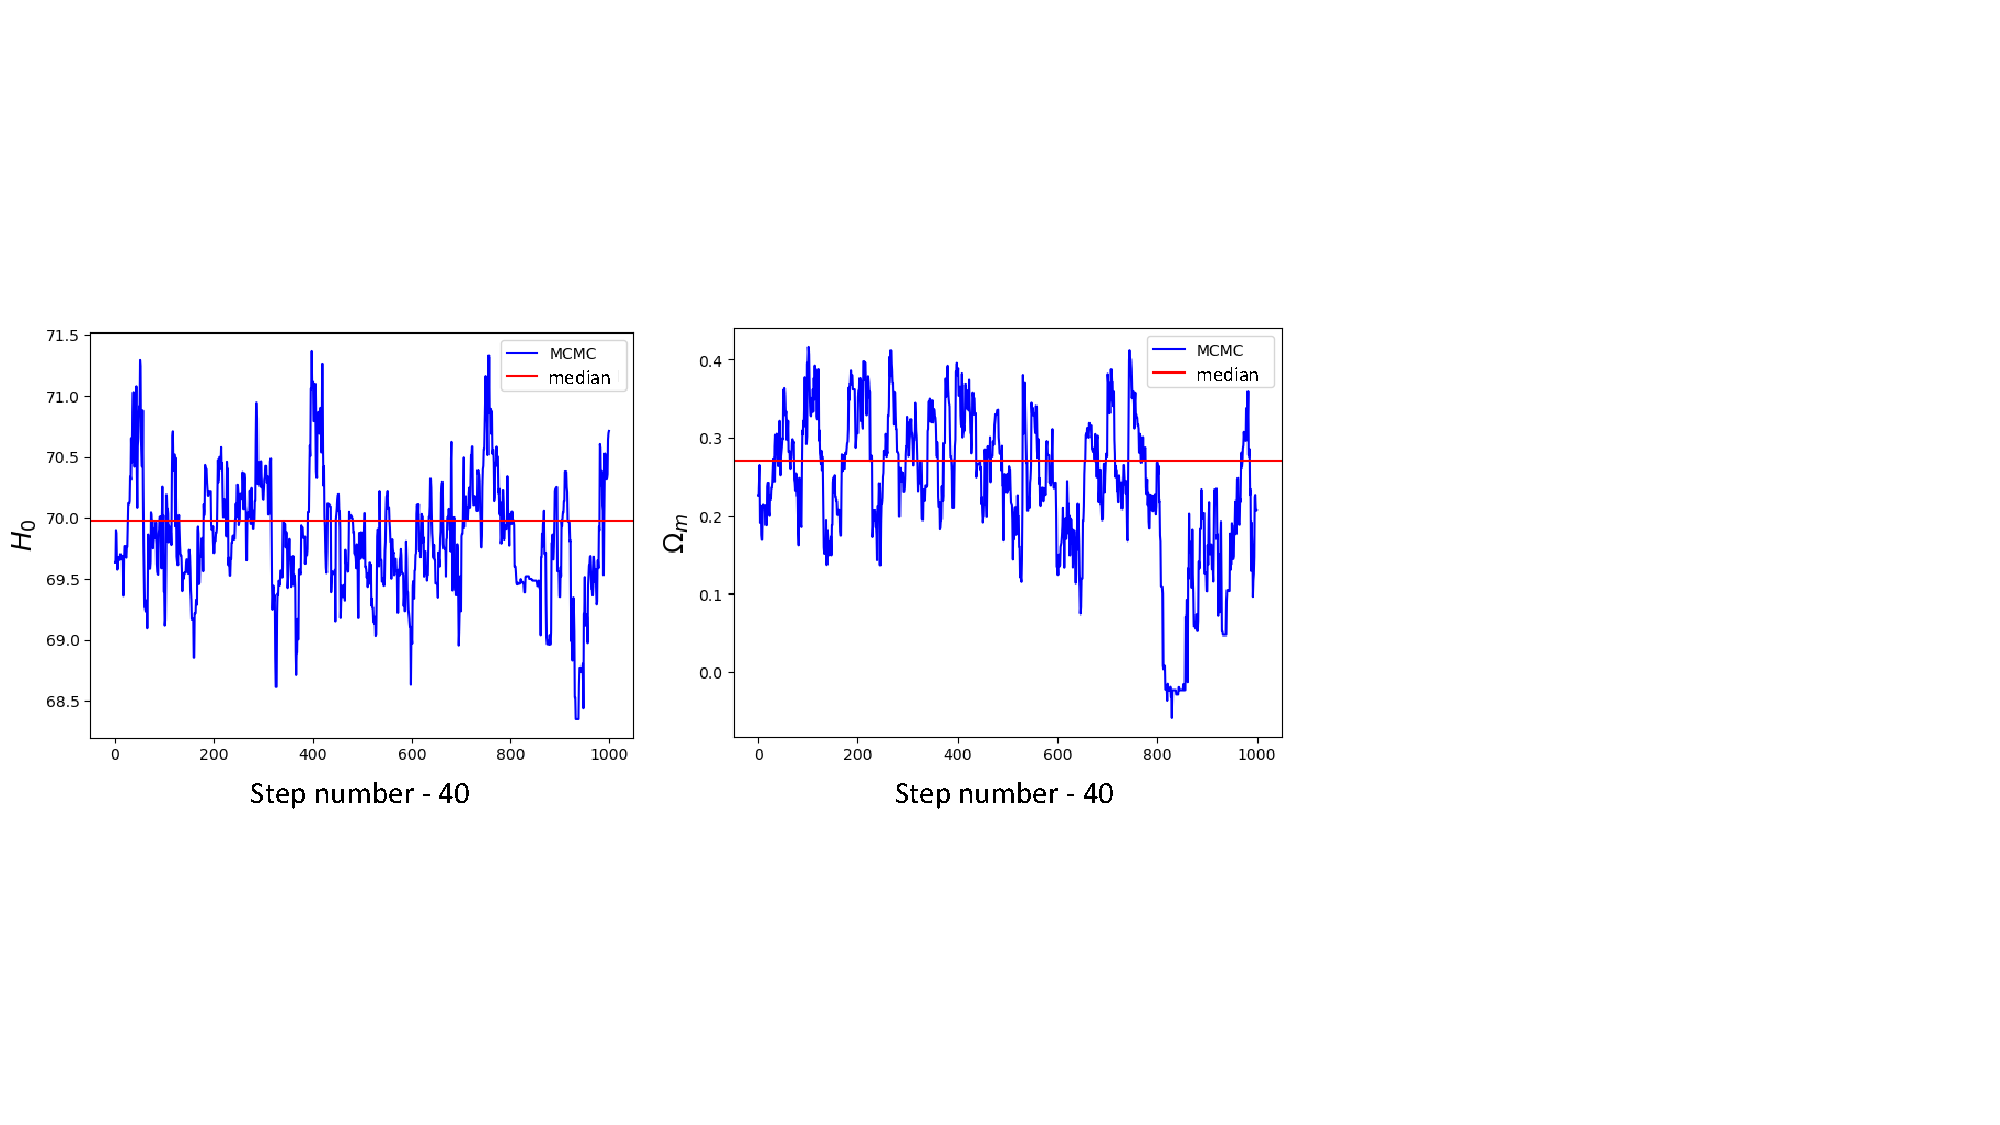
\includegraphics[scale=0.68]{steps1}\\


Figure 2(a) \& 2(b). The average $H_0$- and $\Omega_m$-position of the $20$ walkers.\\
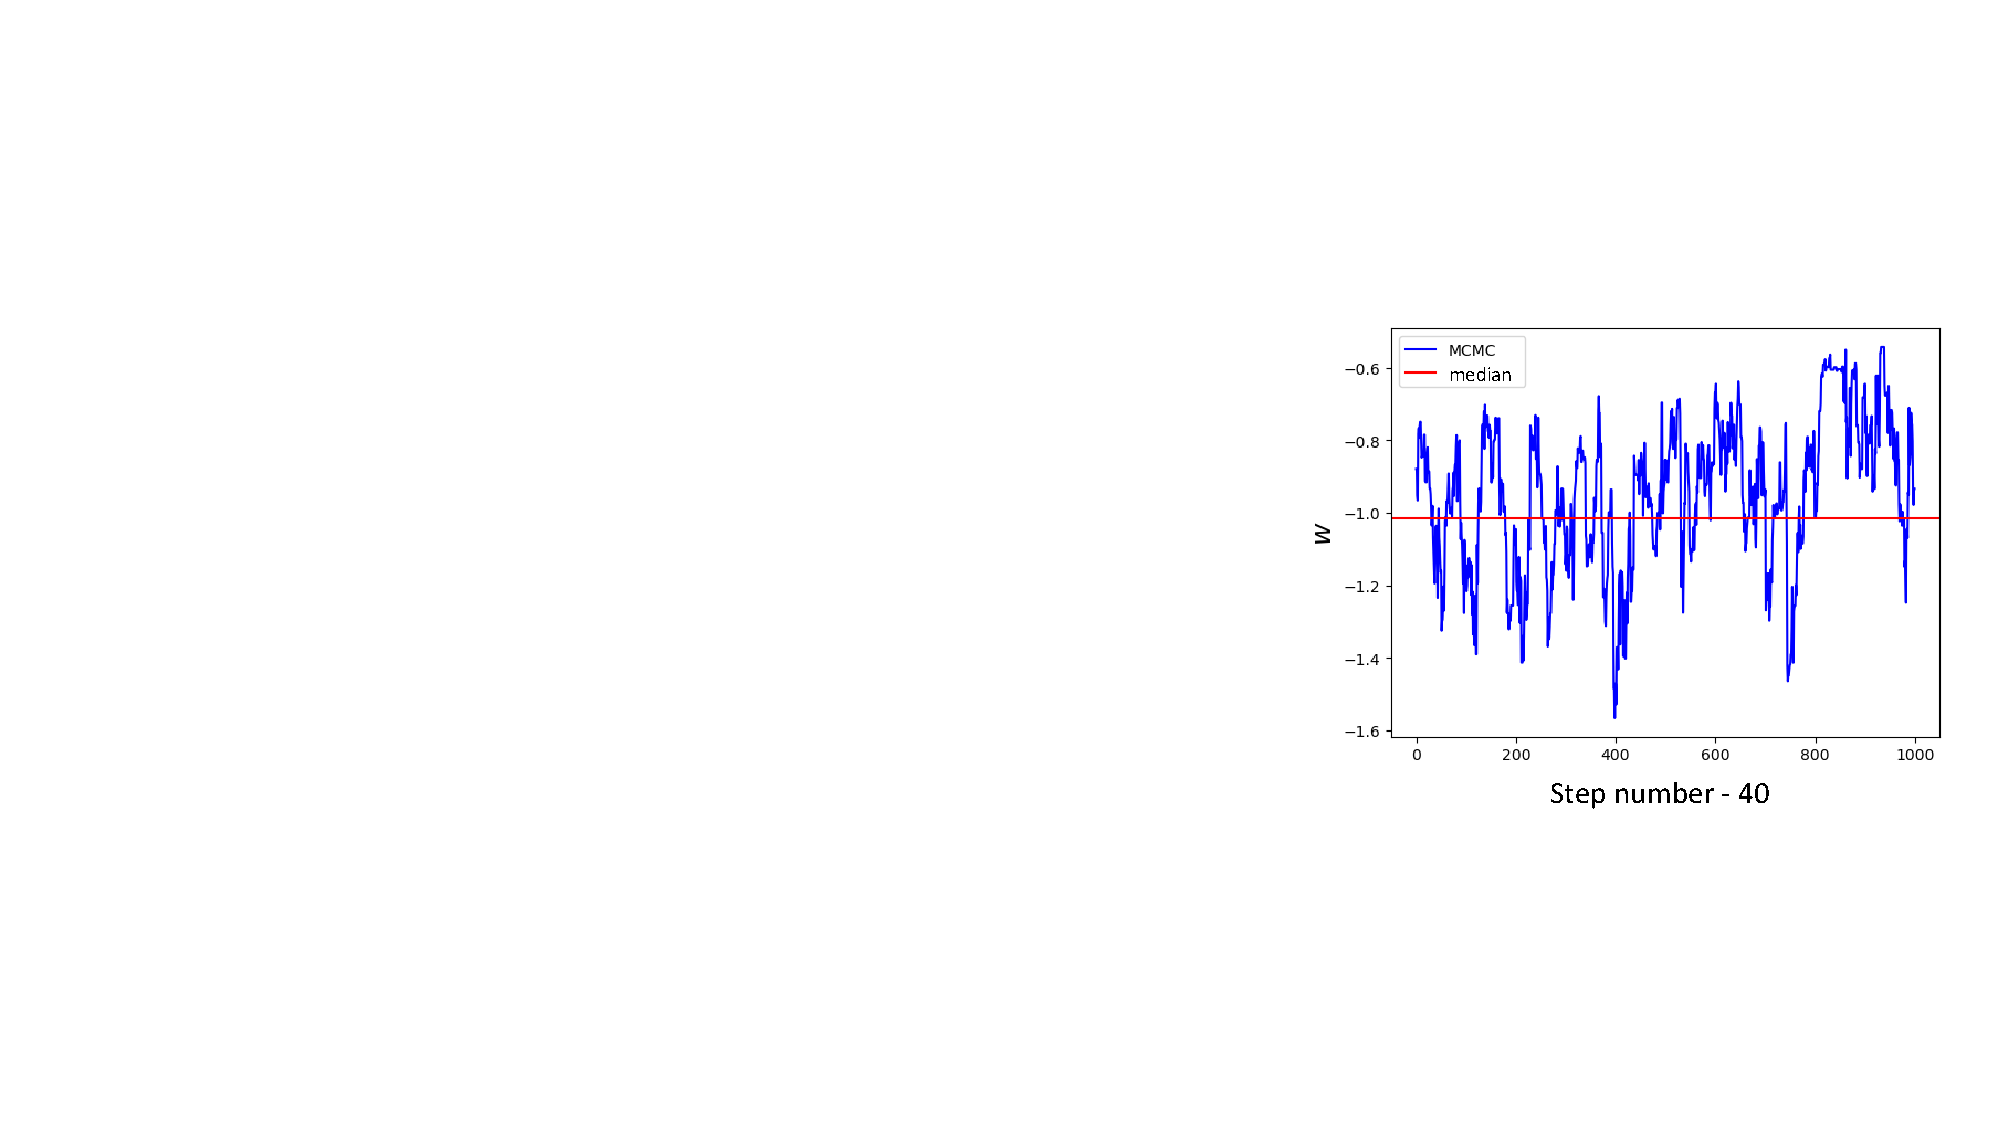
\includegraphics[scale=0.68]{steps2}\\

Figure 2. The average $w$-position of the $20$ walkers. \\

\end{center}
\hfill\break

${}$\qquad Correlation between parameters is displayed in Figure 3 below with [median]\,$\pm $\,[34-percentile] labeled. The values are indeed consistent with the analysis results in the Union 2 and Union 2.1 papers \cite{U21, U2}. \\

\begin{center}
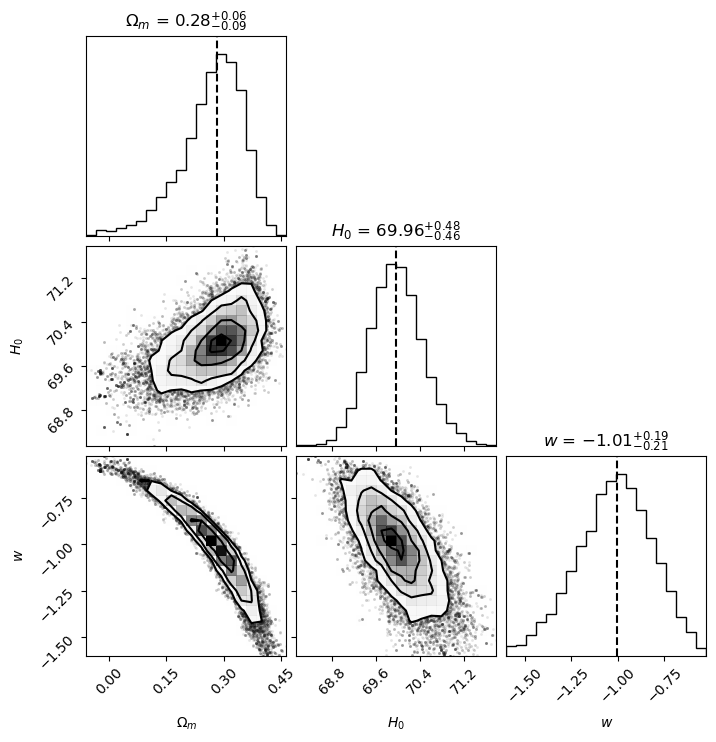
\includegraphics[scale=0.65]{mcmc2}\\
Figure 2. Correlation between parameters and their distributions.
\end{center}

${}$\qquad Using the MCMC method, we have obtained a sample distribution that approximates the posterior $p(\vec{p}\,|X)$, from which we can infer the value of the parameter $\vec{p} = (\Omega_m, w, H_0)$ given the observed data $X$ via elementary statistical argument. Here we choose to use the $16$-$50$-$84$ percentile to interpret the result as the distributions are not normal as observed from Figure 3, and they are not expected to be normal. Since the posterior is a conditional probability distribution of the parameter $\vec{p}$ based on the observed data, by means of \textit{constraining the cosmological parameters}, the occurrence of a cosmological parameter that lies far from the medium, outside the $16$-$84$ percentile or even farther, is interpreted to have a low probability based on our approximation of the posterior.  \\


${}$\qquad Other than the application of MCMC in constraining cosmological parameters in the $\Lambda$CDM model, there is a range of cases in astronomy where MCMC-based Bayesian analysis is making a significant impact. Other examples of the application of MCMC methods in astrophysics include analysis of exoplanets and binary systems using radial velocity measurements, data-driven approach to estimation of stellar parameters from a spectrum, and analysis of solar-like oscillations in stars \cite{Further}. There are also excellent reviews and books on related MCMC-based Bayesian analysis, including R. Trotta's book on \textit{Bayesian Methods in Cosmology} \cite{RT}, and D. Parkinson and A. Liddle's review on \textit{Bayesian Model Averaging in Astrophysics} \cite{AL}. \\

\hfill\break

\noindent\rule{8cm}{1pt}

\bibliography{apssamp}% Produces the bibliography via BibTeX.
\begin{thebibliography}{9}
\bibitem{U21}
N. Suzuki, et al., \textit{The Hubble Space Telescope Cluster Supernova Survey: V. Improving the Dark Energy Constraints Above $z>1$ and Building an Early-Type-Hosted Supernova Sample}, Astrophys. J. \textbf{746}, 85 (2012).
\bibitem{U2}
R. Amanullah, et al., \textit{Spectra and Light Curves of Six Type Ia Supernovae at $0.511 < z < 1.12$ and the Union2 Compilation}, Astrophys. J. \textbf{716}, 712-738 (2010). 
\bibitem{txt}
G. R. Grimmett and D. R. Stirzaker, \textit{Probability and Random Processes} (Oxford University Press, Oxford, United Kingdom, 2001).
\bibitem{Duke}
C. Chan and J. McCarthy, STA-663-2017 1.0 documentation, Duke University, Durham, North Carolina, 2017. The document is available on \url{https://people.duke.edu/~ccc14/sta-663-2017/#}.
\bibitem{ML}
C. Andrieu, N. De Freitas, A. Doucet, and M. I. Jordan,
\textit{An Introduction to MCMC for Machine Learning}, Mach. Learn. \textbf{50}, 5-43 (2003).
\bibitem{Further}
S. Sharma, \textit{Markov Chain Monte Carlo Methods for Bayesian Data Analysis in Astronomy}, Annu. Rev. Astron. Astrophys. \textbf{55}, 213-259 (2017). 
\bibitem{RT}
R. Trotta, \textit{Bayesian Methods in Cosmology} (Imperial College London, Imperial Centre for Inference and Cosmology \& Data Science Institute,
Blackett Laboratory, London, United Kingdom, 2017).
\bibitem{AL}
D. Parkinson and A. Liddle, \textit{Bayesian Model Averaging in Astrophysics: A Review}, Stat. Anal. Data Min. \textbf{6(1)}, 3-14 (2013). 
\end{thebibliography}




\end{document}


